\begin{frame}
  \begin{center}
    \Large{Machine learning}
  \end{center}
\end{frame}

% TODO ? graph with pictures of digits on the x-axis and their corresponding digit
% on the y-axis
\begin{frame}
  \begin{center}
    \includegraphics[scale=0.45]{./pictures/polynomials.png}
  \end{center}
\end{frame}

\begin{frame}
  \begin{center}
  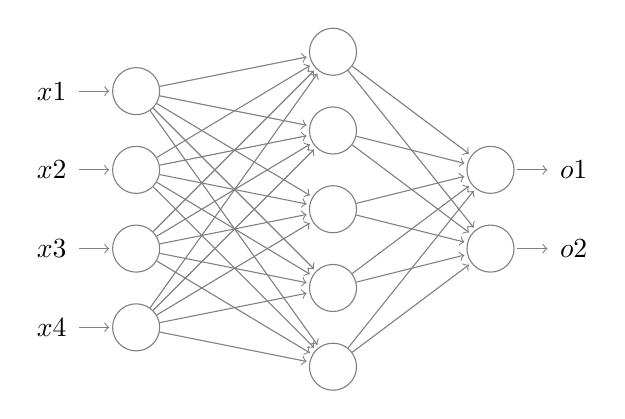
\begin{tikzpicture}[shorten >=1pt,->,draw=black!50, node distance=2.5cm]
    \tikzstyle{every pin edge}=[<-,shorten <=1pt]
    \tikzstyle{neuron}=[circle,draw,minimum size=17pt,inner sep=0pt]

    % input layer nodes
    \foreach \y in {1,...,4}
    \node[neuron, pin=left:$x\y$] (I-\y) at (0,-\y) {};

    % hidden layer nodes
    \foreach \y in {1,...,5}
    \path[yshift=0.5cm]
    node[neuron] (H-\y) at (2.5,-\y) {};

    % output layer node
    \foreach \y in {1,2}
    \path[yshift=-1cm]
    node[neuron,pin={[pin edge={->}]right:$o\y$}] (O-\y) at (4.5,-\y) {};

    % Connect every node in the input layer with every node in the
    % hidden layer.
    \foreach \src in {1,...,4}
    \foreach \dst in {1,...,5}
    \path (I-\src) edge (H-\dst);

    % Connect every node in the hidden layer with the output layer
    \foreach \src in {1,...,5}
    \foreach \dst in {1,2}
    \path (H-\src) edge (O-\dst);
  \end{tikzpicture}
  \end{center}
\end{frame}

%\begin{frame}
  %\frametitle{Prerequisites}
  %\begin{itemize}
    %\item Derivative of composed functions
    %\item Matrix multiplication
    %\item Some python
  %\end{itemize}
%\end{frame}

%\begin{frame}
  %\frametitle{Derivative of composed functions}
  %\begin{equation*}
    %\begin{split}
      %f(g(h(x)))' & = f'(g(h(x))) g'(h(x)) h'(x) \\
      %& = \frac{d f}{d g} \cdot \frac{d g}{d h} \cdot \frac{d h}{d x}
    %\end{split}
  %\end{equation*}
%\end{frame}

%\begin{frame}
  %\frametitle{Matrix multiplication}
  %$
  %\begin{array}{cc}
    %&
    %\left(
      %\begin{matrix}
        %b_{11} & \ldots & b_{12} \\
        %\vdots & \ddots & \vdots \\
        %b_{n1} & \ldots & b_{np}
      %\end{matrix}
    %\right) \\
    %&\\
    %\left(
      %\begin{matrix}
        %a_{11} & \ldots & a_{1n} \\
        %\vdots & \ddots & \vdots \\
        %a_{m1} & \ldots & a_{mn}
      %\end{matrix}
    %\right) & \left(
      %\begin{matrix}
        %c_{11} & \ldots & c_{1p} \\
        %\vdots & \ddots & \vdots \\
        %c_{m1} & \ldots & c_{mp}
      %\end{matrix}
    %\right)
  %\end{array}
  %\qquad c_{ij} = \displaystyle\sum_{k=1}^n{a_{ik} b_{kj}}
  %$
%\end{frame}

%\begin{frame}[fragile]
  %\frametitle{Python}
  %\begin{block}{}
    %\begin{lstlisting}
%def foo(x):
    %l1 = [1, 2, 3, 4]
    %l2 = [5, 6, 7, 8]
    %for elt in l:
        %print(x + elt)
    %for i in range(len(l1)):
        %print(x * l1[i] + l2[i])
    %\end{lstlisting}
  %\end{block}
%\end{frame}

%\begin{frame}[fragile]
  %\frametitle{Numpy}
  %\begin{block}{}
    %\begin{lstlisting}
%from numpy import matrix

%a = matrix([
    %[1, 2, 3],
    %[4, 5, 6]]
%b = matrix([
    %[6, 5],
    %[4, 3],
    %[2, 1]])
%c = a * b
    %\end{lstlisting}
  %\end{block}
%\end{frame}
